\section{Ejemplo 3}

    \lipsum[1]

    \begin{figure}[h]
        \centering
        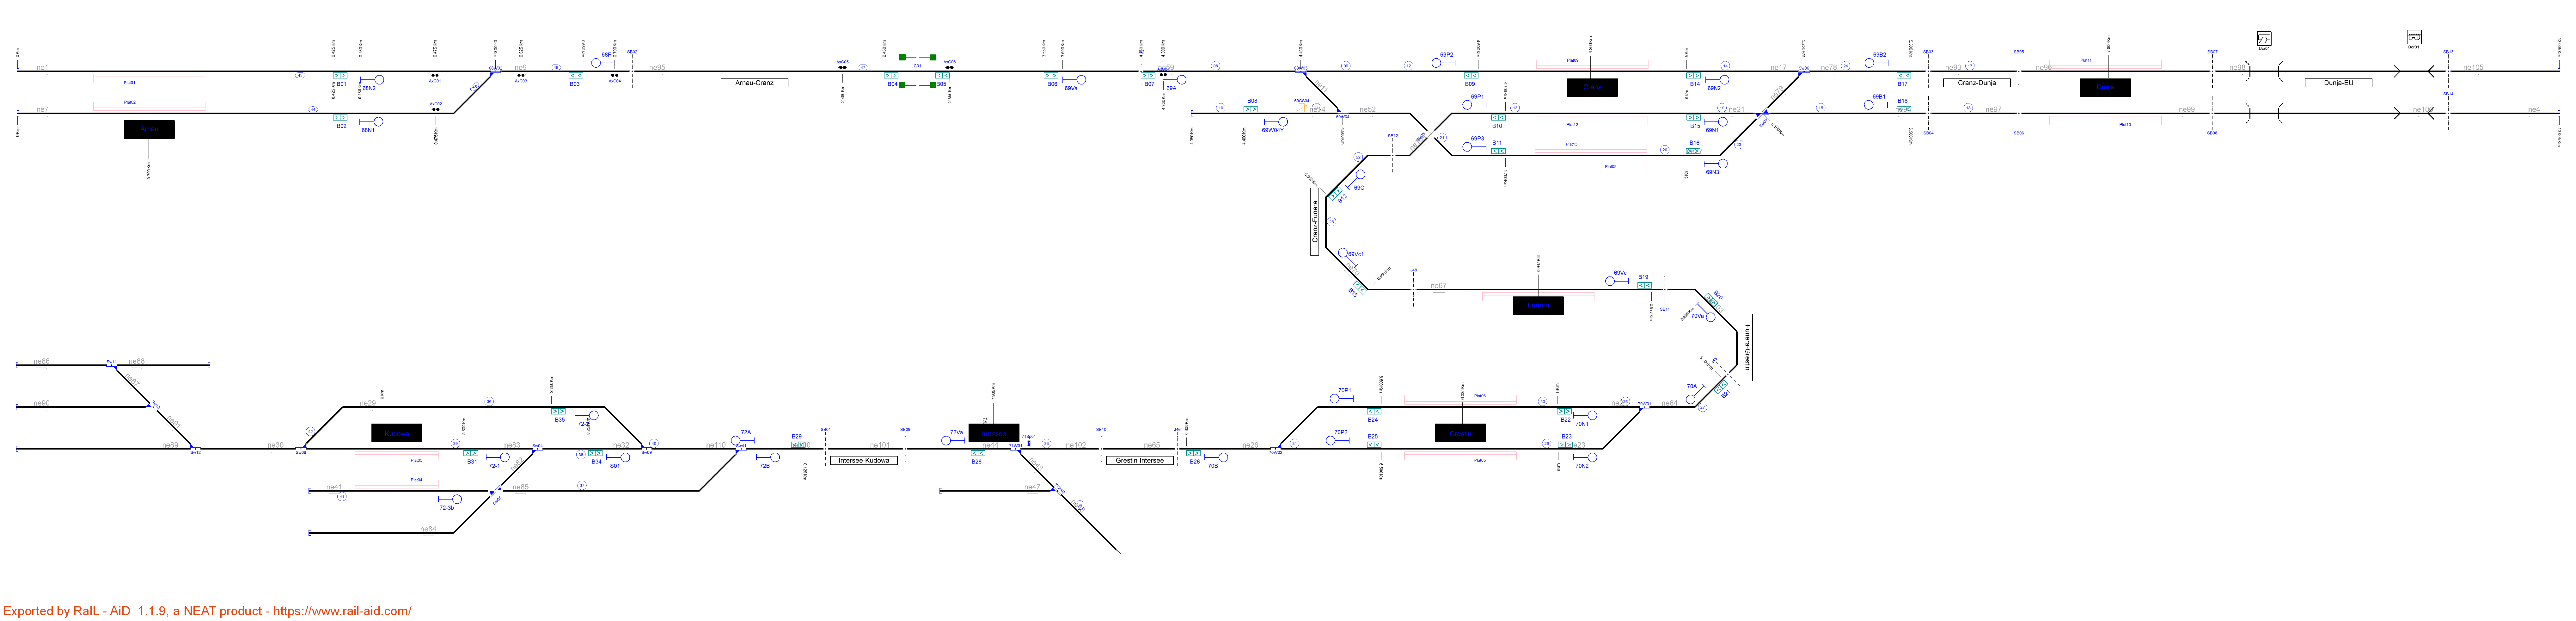
\includegraphics[width=1\textwidth]{resultados-obtenidos/ejemplo3/images/3_original.png}
        \centering\caption{Señalamiento original del ejemplo 3.}
        %\label{fig:LC_P2}
    \end{figure}

    \begin{figure}[h]
        \centering
        
\includegraphics[width=1\textwidth]{resultados-obtenidos/ejemplo3/images/3_empty.png}
        \centering\caption{Topología ferroviaria del ejemplo 3 sin señalamiento.}
        %\label{fig:LC_P2}
    \end{figure}

    \begin{figure}[h]
        \centering
        
\includegraphics[width=1\textwidth]{resultados-obtenidos/ejemplo3/images/3_step1.png}
        \centering\caption{Señalamiento generado por el RNA para proteger el fín de vía.}
        %\label{fig:LC_P2}
    \end{figure}

    \begin{figure}[h]
        \centering
        
\includegraphics[width=1\textwidth]{resultados-obtenidos/ejemplo3/images/3_step2.png}
        \centering\caption{Señalamiento generado por el RNA para proteger las junturas.}
        %\label{fig:LC_P2}
    \end{figure}

    \begin{figure}[h]
        \centering
        
\includegraphics[width=1\textwidth]{resultados-obtenidos/ejemplo3/images/3_step3.png}
        \centering\caption{Señalamiento generado por el RNA para proteger plataformas y cruces de vía.}
        %\label{fig:LC_P2}
    \end{figure}

    \begin{figure}[h]
        \centering
        
\includegraphics[width=1\textwidth]{resultados-obtenidos/ejemplo3/images/3_step4.png}
        \centering\caption{Señalamiento generado por el RNA para proteger las máquinas de cambios.}
        %\label{fig:LC_P2}
    \end{figure}

    \begin{figure}[h]
        \centering
        
\includegraphics[width=1\textwidth]{resultados-obtenidos/ejemplo3/images/3_RNA.png}
        \centering\caption{Señalamiento generado y simplificado por el RNA.}
        %\label{fig:LC_P2}
    \end{figure}

    \subsection{Señalamiento original}

    \lipsum[1]
    
    \begin{table}[H]
        {
        \caption{Tabla de enclavamiento original del ejemplo 3.}
        \label{Tab:tabla_original_3}
        \centering
        \resizebox{1\textwidth}{!}{
            \begin{tabular}{ c c c c c c c }
                \hline	
                    Ruta & Inicio & Final & Cambio & Plataforma & Cruce & netElement \\	
                \hline
                    R$_{01}$ & 68N1 & 69Va & - & - & Lc$_{01}$ & ne$_{7}$-ne$_{95}$\\
                    R$_{02}$ & 68N2 & 69Va & - & - & Lc$_{01}$ & ne$_{1}$-ne$_{95}$\\
                    R$_{03}$ & 69Va & 69A & - & - & - & ne$_{95}$-ne$_{59}$\\
                    R$_{04}$ & 69A & 69N2 & 69W$_{03}^{N}$ & Plat$_{09}$ & - & ne$_{59}$-ne$_{17}$\\
                    R$_{05}$ & 69A & 69N3 & 69W$_{03}^{R}$ & Plat$_{13}$ & - & ne$_{59}$-ne$_{77}$\\
                    R$_{06}$ & 69P2 & 68F & - & - & - & ne$_{17}$-ne$_{9}$\\
                    R$_{07}$ & 69B2 & 69P2 & Sw$_{06}^{N}$ & Plat$_{09}$ & - & ne$_{78}$-ne$_{17}$\\
                    R$_{08}$ & 69B2 & 69P3 & Sw$_{06}^{R}$+Sw$_{07}^{S}$ & Plat$_{13}$ & - & ne$_{78}$-ne$_{77}$\\
                    R$_{09}$ & 69B2 & 69P1 & Sw$_{06}^{R}$+Sw$_{07}^{T}$ & Plat$_{12}$ & - & ne$_{78}$-ne$_{21}$\\
                    R$_{10}$ & 69C & 69N1 & - & Plat$_{12}$ & - & ne$_{70}$-ne$_{21}$\\
                    R$_{11}$ & 69Vc1 & 69C & - & - & -  & ne$_{70}$-ne$_{70}$\\
                    R$_{12}$ & 69Vc & 69Vc1 & - & Plat$_{07}$ & - & ne$_{67}$-ne$_{70}$\\
                    R$_{13}$ & 70Va & 70A & - & - & -  & ne$_{103}$-ne$_{64}$\\
                    R$_{14}$ & 70N2 & 69Vc & - & - & -  & ne$_{23}$-ne$_{67}$\\
                    R$_{15}$ & 70N1 & 69Vc & - & - & - & ne$_{24}$-ne$_{67}$\\
                    R$_{16}$ & 70P1 & 72Va & - & - & - & ne$_{24}$-ne$_{44}$\\
                    R$_{17}$ & 70P2 & 72Va & - & - & - & ne$_{23}$-ne$_{44}$\\
                    R$_{18}$ & 70B & 70N2 & 70W$_{02}^{N}$ & Plat$_{05}$ & - & ne$_{26}$-ne$_{23}$\\
                    R$_{19}$ & 70B & 70N1 & 70W$_{02}^{R}$ & Plat$_{06}$ & - & ne$_{26}$-ne$_{24}$\\
                    R$_{20}$ & 70A & 70P1 & 70W$_{01}^{N}$ & Plat$_{06}$ & - & ne$_{64}$-ne$_{24}$\\
                    R$_{21}$ & 70A & 70P2 & 70W$_{01}^{R}$ & Plat$_{05}$ & - & ne$_{64}$-ne$_{23}$\\
                    R$_{22}$ & 69W04Y & 69N3 & - & Plat$_{13}$ & - & ne$_{14}$-ne$_{77}$\\
                    R$_{23}$ & 72Va & 72A & - & - & - & ne$_{44}$-ne$_{100}$\\
                    R$_{24}$ & 721 & S01 & - & - & - & ne$_{83}$-ne$_{32}$\\
                    R$_{25}$ & 723b & S01 & Sw$_{05}^{T}$ & - & - & ne$_{41}$-ne$_{32}$\\
                    R$_{26}$ & 723b & 72B & Sw$_{05}^{S}$ & - & - & ne$_{41}$-ne$_{100}$\\
                    R$_{27}$ & 722 & 72B & - & - & - & ne$_{29}$-ne$_{100}$\\
                    R$_{28}$ & S01 & 72B & - & - & - & ne$_{32}$-ne$_{100}$\\
                    R$_{29}$ & 69B1 & 69P3 & Sw$_{07}^{T}$ & Plat$_{13}$ & - & ne$_{94}$-ne$_{77}$\\
                    R$_{30}$ & 69B1 & 69P1 & Sw$_{07}^{S}$ & Plat$_{12}$ & - & ne$_{94}$-ne$_{21}$\\
                    R$_{31}$ & 72B & 70B & 71W$_{01}^{N}$ & - & - & ne$_{100}$-ne$_{26}$\\
                    R$_{32}$ & 69P3 & 68F & 69W$_{04}^{R}$ & - & - & ne$_{77}$-ne$_{9}$\\
                    R$_{33}$ & 69P1 & 70Va & - & - & - & ne$_{21}$-ne$_{103}$\\
                \hline
            \end{tabular}
        }
     }
    \end{table}
    
    \lipsum[1]
    \subsection{Señalamiento generado por el RNA}

    \lipsum[1]
    
    \begin{table}[H]
        {
        \caption{Tabla de enclavamiento del ejemplo 3 generada por el RNA (Rutas 1 a 15).}
        \label{Tab:tabla_generated_3_1}
        \centering
        \resizebox{1\textwidth}{!}{
            \begin{tabular}{ c c c c c c c }
                \hline	
                    Ruta & Inicio & Final & Cambio & Plataforma & Cruce & netElement\\	
                \hline
                    R$_{01}$ & T02 & C78 & - & Plat$_{01}$ & - & ne$_{1}$-ne$_{1}$\\
                    R$_{02}$ & T06 & J43 & - & Plat$_{02}$ & - & ne$_{7}$-ne$_{7}$\\
                    R$_{03}$ & T08 & P77 & 69W$_{04}^{N}$ & Plat$_{08}$ & - & ne$_{14}$-ne$_{77}$\\
                    R$_{04}$ & T10 & C100 & Sw$_{04}^{R}$ & Plat$_{04}$ & - & ne$_{41}$-ne$_{32}$\\
                    R$_{05}$ & T10 & S105 & Sw$_{41}^{R}$ & Plat$_{04}$ & - & ne$_{41}$-ne$_{44}$\\
                    R$_{06}$ & T12 & L29 & 71W$_{02}^{R}$ & - & - & ne$_{47}$-ne$_{48}$\\
                    R$_{07}$ & T14 & C100 & Sw$_{04}^{R}$ & - & - & ne$_{84}$-ne$_{32}$\\
                    R$_{08}$ & T14 & S105 & Sw$_{41}^{R}$ & - & - & ne$_{84}$-ne$_{44}$\\
                    R$_{09}$ & T20 & S97 & Sw$_{12}^{N}$ & - & - & ne$_{89}$-ne$_{30}$\\
                    R$_{10}$ & T22 & S97 & Sw$_{12}^{R}$+Sw$_{13}^{R}$ & - & - & ne$_{90}$-ne$_{30}$\\
                    R$_{11}$ & T24 & P70 & - & Plat$_{11}$ & - & ne$_{105}$-ne$_{96}$\\
                    R$_{12}$ & L25 & L42 & - & - & - & ne$_{4}$-ne$_{106}$\\
                    R$_{13}$ & L27 & L30 & - & - & - & ne$_{26}$-ne$_{65}$\\
                    R$_{14}$ & L28 & L40 & - & - & - & ne$_{44}$-ne$_{101}$\\
                    R$_{15}$ & L30 & C104 & - & - & - & ne$_{65}$-ne$_{102}$\\
                \hline
            \end{tabular}
        }
     }
    \end{table}

	\lipsum[1]
	
    \begin{table}[H]
        {
        \caption{Tabla de enclavamiento del ejemplo 3 generada por el RNA (Rutas 16 a 30).}
        \label{Tab:tabla_generated_3_2}
        \centering
        \resizebox{1\textwidth}{!}{
            \begin{tabular}{ c c c c c c c }
                \hline	
                    Ruta & Inicio & Final & Cambio & Plataforma & Cruce & netElement\\	
                \hline
                    R$_{16}$ & L32 & P73 & Sw$_{03}^{N}$ & - & - & ne$_{70}$-ne$_{21}$\\
                    R$_{17}$ & L33 & L34 & - & - & - & ne$_{78}$-ne$_{93}$\\
                    R$_{18}$ & L34 & P71 & - & Plat$_{11}$ & - & ne$_{93}$-ne$_{96}$\\
                    R$_{19}$ & L35 & X50 & - & - & - & ne$_{95}$-ne$_{95}$\\
                    R$_{20}$ & L37 & P76 & - & Plat$_{08}$ & - & ne$_{97}$-ne$_{77}$\\
                    R$_{21}$ & L37 & P72 & - & Plat$_{12}$ & - & ne$_{97}$-ne$_{21}$\\
                    R$_{22}$ & L38 & T23 & - & - & - & ne$_{98}$-ne$_{105}$\\
                    R$_{23}$ & L40 & S126 & - & - & - & ne$_{101}$-ne$_{100}$\\
                    R$_{24}$ & L41 & S90 & - & - & - & ne$_{103}$-ne$_{64}$\\
                    R$_{25}$ & L42 & P68 & - & Plat$_{10}$ & - & ne$_{106}$-ne$_{99}$\\
                    R$_{26}$ & J43 & J46 & 68W$_{02}^{R}$ & - & - & ne$_{7}$-ne$_{9}$\\
                    R$_{27}$ & J46 & L35 & - & - & - & ne$_{9}$-ne$_{95}$\\
                    R$_{28}$ & X50 & S83 & - & - & Lc01 & ne$_{95}$-ne$_{59}$\\
                    R$_{29}$ & X51 & S80 & - & - & Lc01 & ne$_{95}$-ne$_{9}$\\
                    R$_{30}$ & P60 & L27 & 70W$_{02}^{N}$ & - & - & ne$_{23}$-ne$_{26}$\\
                \hline
            \end{tabular}
        }
     }
    \end{table}

	\lipsum[1]
	
    \begin{table}[H]
        {
        \caption{Tabla de enclavamiento del ejemplo 3 generada por el RNA (Rutas 31 a 45).}
        \label{Tab:tabla_generated_3_3}
        \centering
        \resizebox{1\textwidth}{!}{
            \begin{tabular}{ c c c c c c c }
                \hline	
                    Ruta & Inicio & Final & Cambio & Plataforma & Cruce & netElement\\	
                \hline
                    R$_{31}$ & P63 & L41 & 70W$_{01}^{N}$ & - & - & ne$_{24}$-ne$_{103}$\\
                    R$_{32}$ & P64 & L32 & - & - & - & ne$_{67}$-ne$_{70}$\\
                    R$_{33}$ & P65 & L41 & - & - & - & ne$_{67}$-ne$_{103}$\\
                    R$_{34}$ & P68 & L37 & - & - & - & ne$_{99}$-ne$_{97}$\\
                    R$_{35}$ & P69 & T03 & - & - & - & ne$_{99}$-ne$_{4}$\\
                    R$_{36}$ & P70 & S110 & - & - & - & ne$_{96}$-ne$_{78}$\\
                    R$_{37}$ & P71 & L38 & - & - & - & ne$_{96}$-ne$_{98}$\\
                    R$_{38}$ & P72 & L32 & - & - & - & ne$_{21}$-ne$_{70}$\\
                    R$_{39}$ & P73 & L33 & Sw$_{06}^{R}$ & - & - & ne$_{21}$-ne$_{78}$\\ 
                    R$_{40}$ & P73 & P69 & - & Plat$_{10}$ & - & ne$_{21}$-ne$_{99}$\\
                    R$_{41}$ & P76 & S86 & - & - & - & ne$_{77}$-ne$_{52}$\\
                    R$_{42}$ & P77 & L33 & Sw$_{06}^{R}$ & - & - & ne$_{77}$-ne$_{78}$\\
                    R$_{43}$ & P77 & P69 &  & Plat$_{10}$ & - & ne$_{77}$-ne$_{99}$\\
                    R$_{44}$ & C78 & J46 & 68W$_{02}^{N}$ & - & - & ne$_{1}$-ne$_{9}$\\
                    R$_{45}$ & S80 & T01 & 68W$_{02}^{N}$ & Plat$_{01}$ & - & ne$_{9}$-ne$_{1}$\\
                \hline
            \end{tabular}
        }
     }
    \end{table}

	\lipsum[1]
	
    \begin{table}[H]
        {
        \caption{Tabla de enclavamiento del ejemplo 3 generada por el RNA (Rutas 46 a 60).}
        \label{Tab:tabla_generated_3_4}
        \centering
        \resizebox{1\textwidth}{!}{
            \begin{tabular}{ c c c c c c c }
                \hline	
                    Ruta & Inicio & Final & Cambio & Plataforma & Cruce & netElement\\	
                \hline
                    R$_{46}$ & S80 & T05 & 68W$_{02}^{R}$ & Plat$_{02}$ & - & ne$_{9}$-ne$_{7}$\\
                    R$_{47}$ & S82 & X51 & 69W$_{03}^{N}$ & - & - & ne$_{17}$-ne$_{95}$\\
                    R$_{48}$ & S83 & P77 & 69W$_{03}^{R}$+69W$_{04}^{R}$ & Plat$_{08}$ & - & ne$_{59}$-ne$_{77}$\\
                    R$_{49}$ & S83 & S109 & 69W$_{03}^{N}$ & Plat$_{09}$ & - & ne$_{59}$-ne$_{17}$\\
                    R$_{50}$ & S86 & X51 & 69W$_{03}^{R}$+69W$_{04}^{R}$ & - & - & ne$_{52}$-ne$_{95}$\\
                    R$_{51}$ & S86 & T07 & 69W$_{04}^{N}$ & - & - & ne$_{52}$-ne$_{14}$\\
                    R$_{52}$ & B89 & L41 & 70W$_{01}^{R}$ & Plat$_{05}$ & - & ne$_{23}$-ne$_{103}$\\
                    R$_{53}$ & S90 & P60 & 70W$_{01}^{R}$ & Plat$_{05}$ & - & ne$_{64}$-ne$_{23}$\\
                    R$_{54}$ & S90 & L27 & 70W$_{01}^{R}$+70W$_{02}^{N}$ & Plat$_{05}$ & - & ne$_{64}$-ne$_{26}$\\
                    R$_{55}$ & B92 & P63 & - & - & - & ne$_{24}$-ne$_{24}$\\
                    R$_{56}$ & S93 & B89 & 70W$_{02}^{N}$ & - & - & ne$_{26}$-ne$_{23}$\\
                    R$_{57}$ & S93 & P92 & 70W$_{02}^{R}$ & Plat$_{06}$ & - & ne$_{26}$-ne$_{24}$\\
                    R$_{58}$ & S95 & S119 & Sw$_{08}^{N}$ & - & - & ne$_{83}$-ne$_{30}$\\
                    R$_{59}$ & S96 & S119 & Sw$_{08}^{R}$ & - & - & ne$_{29}$-ne$_{30}$\\
                    R$_{60}$ & S97 & C124 & Sw$_{08}^{R}$+Sw$_{09}^{R}$ & - & - & ne$_{30}$-ne$_{110}$\\
                \hline
            \end{tabular}
        }
     }
    \end{table}
    
    \lipsum[1]
    
    \begin{table}[H]
        {
        \caption{Tabla de enclavamiento del ejemplo 3 generada por el RNA (Rutas 61 a 75).}
        \label{Tab:tabla_generated_3_5}
        \centering
        \resizebox{1\textwidth}{!}{
            \begin{tabular}{ c c c c c c c }
                \hline	
                    Ruta & Inicio & Final & Cambio & Plataforma & Cruce & netElement\\	
                \hline
                    R$_{61}$ & S97 & C112 & Sw$_{08}^{N}$ & Plat$_{03}$ & - & ne$_{30}$-ne$_{83}$\\
                    R$_{62}$ & C100 & S124 & Sw$_{09}^{N}$ & - & - & ne$_{32}$-ne$_{110}$\\
                    R$_{63}$ & B101 & S96 & - & - & - & ne$_{29}$-ne$_{29}$\\
                    R$_{64}$ & S102 & S113 & Sw$_{09}^{N}$ & - & - & ne$_{110}$-ne$_{32}$\\
                    R$_{65}$ & S102 & B101 & Sw$_{09}^{R}$ & - & - & ne$_{110}$-ne$_{29}$\\
                    R$_{66}$ & C104 & L28 & 71W$_{01}^{N}$ & - & - & ne$_{102}$-ne$_{44}$\\
                    R$_{67}$ & S105 & L29 & 71W$_{01}^{R}$+71W$_{02}^{N}$ & - & - & ne$_{44}$-ne$_{48}$\\
                    R$_{68}$ & S105 & S93 & 71W$_{01}^{N}$ & - & - & ne$_{44}$-ne$_{26}$\\
                    R$_{69}$ & C109 & L33 & Sw$_{06}^{N}$ & - & - & ne$_{17}$-ne$_{78}$\\
                    R$_{70}$ & S110 & S82 & Sw$_{06}^{N}$ & Plat$_{09}$ & - & ne$_{78}$-ne$_{17}$\\
                    R$_{71}$ & S110 & P76 & Sw$_{06}^{R}$ & Plat$_{08}$ & - & ne$_{78}$-ne$_{77}$\\
                    R$_{72}$ & S110 & P72 & Sw$_{06}^{R}$ & Plat$_{12}$ & - & ne$_{78}$-ne$_{21}$\\
                    R$_{73}$ & C112 & C100 & Sw$_{04}^{N}$ & - & - & ne$_{83}$-ne$_{32}$\\
                    R$_{74}$ & S113 & C95 & Sw$_{04}^{N}$ & Plat$_{03}$ & - & ne$_{32}$-ne$_{83}$\\
                    R$_{75}$ & S113 & P58 & Sw$_{04}^{R}$ & Plat$_{04}$ & - & ne$_{32}$-ne$_{41}$\\
                \hline
            \end{tabular}
        }
     }
    \end{table}
    
    \lipsum[1]
    
    \begin{table}[H]
        {
        \caption{Tabla de enclavamiento del ejemplo 3 generada por el RNA (Rutas 75 a 87).}
        \label{Tab:tabla_generated_3_6}
        \centering
        \resizebox{1\textwidth}{!}{
            \begin{tabular}{ c c c c c c c }
                \hline	
                    Ruta & Inicio & Final & Cambio & Plataforma & Cruce & netElement\\	
                \hline
                    R$_{76}$ & S113 & S13 & Sw$_{04}^{R}$ & - & - & ne$_{32}$-ne$_{84}$\\
                    R$_{77}$ & S115 & S15 & Sw$_{11}^{N}$ & - & - & ne$_{88}$-ne$_{86}$\\
                    R$_{78}$ & S116 & S17 & Sw$_{11}^{N}$ & - & - & ne$_{86}$-ne$_{88}$\\
                    R$_{79}$ & S116 & S97 & Sw$_{11}^{R}$+Sw$_{12}^{R}$+Sw$_{13}^{N}$ & - & - & ne$_{86}$-ne$_{30}$\\
                    R$_{80}$ & S119 & S19 & Sw$_{12}^{N}$ & - & - & ne$_{30}$-ne$_{89}$\\
                    R$_{81}$ & S119 & S15 & Sw$_{11}^{R}$+Sw$_{12}^{R}$+Sw$_{13}^{N}$ & - & - & ne$_{30}$-ne$_{86}$\\
                    R$_{82}$ & S119 & S21 & Sw$_{12}^{R}$+Sw$_{13}^{R}$ & - & - & ne$_{30}$-ne$_{90}$\\
                    R$_{83}$ & S124 & S105 & Sw$_{41}^{N}$ & - & - & ne$_{110}$-ne$_{44}$\\
                    R$_{84}$ & S125 & S58 & - & Plat$_{04}$ & - & ne$_{85}$-ne$_{41}$\\
                    R$_{85}$ & S125 & S13 & - & - & - & ne$_{85}$-ne$_{84}$\\
                    R$_{86}$ & S126 & S102 & Sw$_{41}^{N}$ & - & - & ne$_{100}$-ne$_{110}$\\
                    R$_{87}$ & S126 & S125 & Sw$_{41}^{R}$ & - & - & ne$_{100}$-ne$_{85}$\\
                \hline
            \end{tabular}
        }
     }
    \end{table}
    
    \lipsum[1]
    \subsection{Sistema generado por el ACG}

En base a la red de grafos, ilustrada en la Figura \ref{fig:EJ3_8}, el ACG determinó la siguiente cantidad de elementos, tal puede visualizarse en el Código \ref{lst:EJ3_8}.

\begin{lstlisting}[language = {}, caption = Cantidad de elementos a implementar por el ACG, label = {lst:EJ3_8}]
n_netElements:53
n_switch:15
n_doubleSwitch:2
n_borders:18
n_buffers:12
n_levelCrossings:1
n_platforms:13
n_scissorCrossings:1
n_signals:82
N : 329
M : 276
\end{lstlisting}

El código VHDL generado por el ACG es importado en un proyecto de Vivado, donde es sintetizado e implementado para generar el bitstream que será utilizado para programar la FPGA. La cantidad de elementos de la FPGA utilizados por el sistema post-síntesis y post-implementación, así como el porcentaje de uso de la plataforma, son detallados en la Tabla \ref{Tab:tabla_ACG_3}.

\begin{table}[H]
	{
		\caption{Síntesis e implementación del ejemplo 3 generado por el ACG.}
		\label{Tab:tabla_ACG_3}
		\centering
		%\small
		%\centering
		\begin{center}
			\resizebox{0.7\textwidth}{!}{
				\begin{tabular}{ c c c c }
					\hline	
					Recursos & Síntesis & Implementación & Uso \\	
					\hline
					LUT & 13802 & 137873 & 25.94-25.91\%\\
					FF & 17321 & 17321 & 16.28\%\\
					IO & 16 & 16 & 12.80\%\\
					BUFG & 1 & 1 & 3.13\%\\
					\hline
				\end{tabular}
			}
		\end{center}
	}    
\end{table}

En este ejemplo, la cantidad de recursos utilizados es baja y el tiempo de sintetización e implementación es de 1 minuto con 43 segundos y 1 minuto con 20 segundos respectivamente.
    \section{Validación del sistema}

	La validación de las rutas de la tabla de enclavamientos es realizada por el RNA aplicando el Algoritmo \ref{alg:interlocking_tables}, explicado en la Sección \ref{sec:validar_tabla}. Las 33 rutas del señalamiento original (Tabla \ref{Tab:tabla_original_3}) tienen 33 rutas equivalentes en el señalamiento generado por el RNA (Tabla \ref{Tab:tabla_generated_3_1}, \ref{Tab:tabla_generated_3_2}, \ref{Tab:tabla_generated_3_3}, \ref{Tab:tabla_generated_3_4}, \ref{Tab:tabla_generated_3_5}, \ref{Tab:tabla_generated_3_6}), tal como se puede visualizar en la Tabla \ref{Tab:tabla_validation_3_1}, generada automáticamente por el RNA. % y Tabla \ref{Tab:tabla_validation_3_2}, generada automáticamente por el RNA.

    \begin{table}[H]
        {
        \caption{Equivalencias entre las rutas originales y las generadas por el RNA.}
        \label{Tab:tabla_validation_3_1}
        \centering
        %\small
            %\centering
            \begin{center}
            \resizebox{0.9\textwidth}{!}{
            \begin{tabular}{ c c c c }
                \hline	
                    Original & Señales & RNA & Señales \\	
                \hline
                    R$_{01}$ & 68N1-69Va & R$_{23}$+R$_{24}$ & J$_{43}$-L$_{35}$\\
                    R$_{02}$ & 68N2-69Va & R$_{38}$+R$_{24}$ & C$_{78}$-L$_{35}$\\
                    R$_{03}$ & 69Va-69A & R$_{25}$ & X$_{50}$-S$_{83}$\\
                    R$_{04}$ & 69A-69N2 & R$_{43}$ & S$_{83}$-S$_{109}$\\
                    R$_{05}$ & 69A-69N3 & R$_{42}$+R$_{91}$ & S$_{83}$-B$_{145}$\\
                    R$_{06}$ & 69P2-68F & R$_{41}$+R$_{26}$ & S$_{82}$-S$_{80}$\\
                    R$_{07}$ & 69B2-69P2 & R$_{64}$ & S$_{110}$-S$_{82}$\\
                    R$_{08}$ & 69B2-69P3 & R$_{65}$ & S$_{110}$-B$_{133}$\\
                    R$_{09}$ & 69B2-69P1 & R$_{66}$ & S$_{110}$-P$_{72}$\\
                    R$_{10}$ & 69C-69N1 & R$_{14}$ & L$_{32}$-T$_{73}$\\
                    R$_{11}$ & 69Vc1-69C & R$_{88}$+R$_{87}$ & S$_{144}$-L$_{32}$\\
                    R$_{12}$ & 69Vc-69Vc1 & R$_{29}$ & P$_{64}$-L$_{32}$\\
                    R$_{13}$ & 70Va-70A & R$_{21}$ & L$_{41}$-S$_{90}$\\
                    R$_{14}$ & 70N2-69Vc & R$_{27}$ & P$_{60}$-L$_{27}$\\
                    R$_{15}$ & 70N1-69Vc & R$_{28}$ & P$_{63}$-L$_{41}$\\
                    R$_{16}$ & 70P1-72Va & R$_{28}$+R$_{21}$+R$_{48}$+R$_{11}$+R$_{13}$+R$_{60}$ & P$_{63}$-L$_{28}$\\
    %            \hline
    %        \end{tabular}
    %        }
    %        \end{center}
    %    }    
    %\end{table}

	%\lipsum[1]
	
    %\begin{table}[H]
    %    {
    %    \caption{Equivalencias entre las rutas originales y las generadas por el RNA (Rutas 17 a 33).}
    %    \label{Tab:tabla_validation_3_2}
    %    \centering
        %\small
            %\centering
   %         \begin{center}
   %         \resizebox{0.8\textwidth}{!}{
   %         \begin{tabular}{ c c c c }
   %             \hline	
   %                 Original & Señales & RNA & Señales \\	
   %             \hline
                    R$_{17}$ & 70P2-72Va & R$_{27}$+R$_{11}$+R$_{13}$+R$_{60}$ & P$_{60}$-L$_{28}$\\
                    R$_{18}$ & 70B-70N2 & R$_{50}$ & S$_{93}$-B$_{89}$\\
                    R$_{19}$ & 70B-70N1 & R$_{51}$ & S$_{93}$-P$_{92}$\\
                    R$_{20}$ & 70A-70P1 & R$_{48}$+R$_{51}$ & S$_{90}$-P$_{92}$\\
                    R$_{21}$ & 70A-70P2 & R$_{47}$ & S$_{90}$-P$_{60}$\\
                    R$_{22}$ & 69W04Y-69N3 & R$_{03}$+R$_{91}$ & T$_{08}$-B$_{145}$\\
                    R$_{23}$ & 72Va-72A & R$_{12}$+R$_{20}$ & L$_{28}$-S$_{139}$\\
                    R$_{24}$ & 721-S01 & R$_{67}$ & C$_{114}$-C$_{100}$\\
                    R$_{25}$ & 723b-S01 & R$_{77}$ & B$_{130}$-C$_{100}$\\
                    R$_{26}$ & 723b-72B & R$_{78}$+R$_{12}$+R$_{20}$ & B$_{130}$-S$_{139}$\\
                    R$_{27}$ & 722-72B & R$_{53}$+R$_{54}$+R$_{84}$+R$_{12}$+R$_{20}$ & S$_{96}$-S$_{122}$\\
                    R$_{28}$ & S01-72B & R$_{70}$+R$_{06}$+R$_{12}$+R$_{20}$ & S$_{113}$-S$_{122}$\\
                    R$_{29}$ & 69B1-69P3 & R$_{82}$ & S$_{135}$-B$_{133}$\\
                    R$_{30}$ & 69B1-69P1 & R$_{83}$ & S$_{135}$-P$_{72}$\\
                    R$_{31}$ & 72B-70B & R$_{85}$+R$_{84}$+R$_{62}$ & S$_{139}$-S$_{93}$\\
                    R$_{32}$ & 69P3-68F & R$_{81}$+R$_{44}$+R$_{26}$ &B$_{133}$-S$_{80}$\\
                    R$_{33}$ & 69P1-70Va & R$_{36}$ & P$_{73}$-L$_{33}$\\
                \hline
            \end{tabular}
            }
            \end{center}
        }    
    \end{table}
    
    Las rutas R1, R2, R5, R6, R11, R16, R17, R20, R22, R23, R26, R27, R28, R31 y R32 del señalamiento original fueron divididas en rutas mas pequeñas en el señalamiento generado por el RNA. La razón para dividir la ruta depende de cada caso, tal sea por su longitud y/o por abarcar diversos elementos ferroviarios. Por ejemplo, la ruta R32 fue dividida por ambos motivos: es muy extensa y atraviesa un cambio de vías en tijeras, dos cambios de vías simples, un cruce de vías y una plataforma. Las rutas producto de particionar R32 (R81, R44 y R26 del nuevo señalamiento) añaden paradas luego de cruzar el cambio de vías en tijeras y antes del cruce de vías, incrementando la seguridad y flexibilidad en la logística de la red. Un análisis similar puede hacerse con las demás rutas particionadas.
    
    De las 91 rutas generadas por el RNA, 29 son particiones de rutas originales, por lo que 62 de ellas están relacionadas de alguna manera a las 33 rutas originales. Las 29 rutas restantes corresponden a la protección de los 12 finales de vía absolutos y al único final de vía relativo, además de las señales añadidas para poder operar las playas de maniobras que se encontraban sin señalamiento.
    
    Para finalizar, el RNA comprueba los principios de señalamiento ferroviario explicados en la Sección \label{sec:validar_principios}, aplicando los algoritmos indicados, de los cuáles se obtuvieron los siguientes resultados:
    
    \begin{itemize}
    	\item Principio de autoridad (Algoritmo \ref{alg:ppio_autoridad}): cobertura del 100\% de los \textit{netElements}.
    	\item Principio de claridad (Algoritmo \ref{alg:ppio_claridad}): rutas 100\% independientes.
    	\item Principio de anticipación (Algoritmo \ref{alg:ppio_anticipacion}): cobertura del 100\% de los puntos críticos.
    	\item Principio de granularidad (Algoritmo \ref{alg:ppio_granularidad}): 100\% de rutas divididas a su mínima expresión.
    	\item Principio de terminalidad (Algoritmo \ref{alg:ppio_terminalidad}): 100\% de finales de vías protegidos.
    	\item Principio de infraestructura (Algoritmo \ref{alg:ppio_infraestructura}): 100\% de infraestructura protegida.
    	\item Principio de no bloqueo (Algoritmo \ref{alg:ppio_nobloqueo}): 100\% de cambios de vías protegidos.
    \end{itemize}	